% This must be in the first 5 lines to tell arXiv to use pdfLaTeX, which is strongly recommended.
\pdfoutput=1
% In particular, the hyperref package requires pdfLaTeX in order to break URLs across lines.

\documentclass[11pt]{article}

% Change "review" to "final" to generate the final (sometimes called camera-ready) version.
% Change to "preprint" to generate a non-anonymous version with page numbers.
\usepackage[review]{acl}
% Standard package includes
\usepackage{times}
\usepackage{latexsym}
\usepackage{graphicx}

\usepackage{algorithmic}
\usepackage{algorithm}
\usepackage{multirow}
\usepackage{natbib}
\usepackage{subcaption}

% For proper rendering and hyphenation of words containing Latin characters (including in bib files)
\usepackage[T1]{fontenc}
% For Vietnamese characters
% \usepackage[T5]{fontenc}
% See https://www.latex-project.org/help/documentation/encguide.pdf for other character sets

% This assumes your files are encoded as UTF8
\usepackage[utf8]{inputenc}
\usepackage[export]{adjustbox}

% This is not strictly necessary, and may be commented out,
% but it will improve the layout of the manuscript,
% and will typically save some space.
\usepackage{microtype}
\usepackage{hyperref}

% This is also not strictly necessary, and may be commented out.
% However, it will improve the aesthetics of text in
% the typewriter font.
\usepackage{inconsolata}
% If the title and author information does not fit in the area allocated, uncomment the following
%
%\setlength\titlebox{<dim>}
%
% and set <dim> to something 5cm or larger.
\newcommand{\secref}[1]{Sec. \ref{#1}}
\newcommand{\figref}[1]{Figure \ref{#1}}
\newcommand{\eqnref}[1]{Eq. (\ref{#1})}
\newcommand{\tabref}[1]{Table \ref{#1}}
\newcommand{\exref}[1]{Example \ref{#1}}
\newcommand{\ZZ}[1]{\textcolor{brown}{(Zander: #1})}
\newcommand{\KZ}[1]{\textcolor{blue}{(Kenny: #1})}
\newcommand{\MY}[1]{\textcolor{red}{(Mengyue: #1})}

\title{PersonaMovs: A Multimedia Conversational Dataset for Dynamic Personality Analysis}

% Author information can be set in various styles:
% For several authors from the same institution:
% \author{Author 1 \and ... \and Author n \\
%         Address line \\ ... \\ Address line}
% if the names do not fit well on one line use
%         Author 1 \\ {\bf Author 2} \\ ... \\ {\bf Author n} \\
% For authors from different institutions:
% \author{Author 1 \\ Address line \\  ... \\ Address line
%         \And  ... \And
%         Author n \\ Address line \\ ... \\ Address line}
% To start a separate ``row'' of authors use \AND, as in
% \author{Author 1 \\ Address line \\  ... \\ Address line
%         \AND
%         Author 2 \\ Address line \\ ... \\ Address line \And
%         Author 3 \\ Address line \\ ... \\ Address line}




\begin{document}
\maketitle
\begin{abstract}
Automatic personality detection has evolved from simple text classification to sophisticated multimodal analysis, recognizing the multidimensional manifestation of personality beyond textual data. This shift highlights the need for datasets that can accurately capture the complexity of human personality through diverse modalities. We introduce the PersonaMovs (PM), a large, extensive and varied multimedia conversational dataset, built on 305 movies and 14 TV series, featuring over 46k dialogues, 552k utterances, 4016 characters, and 963 hours of video. PM not only addresses the challenges of existing datasets by offering majority-voted personality annotations and detailed relations networks but also paves the way for advanced analysis of personality dynamics across various contexts.
\end{abstract}
\section{Introduction}

Protein$-$protein interactions (PPIs) are of central importance for the majority of biological functions, such as signal transduction, metabolic pathways, molecular dynamics, and protein networks\cite{Hoffmann.Krallinger.ea:2005}, for they serve as the most fundamental building blocks of the entire interacademic systems of any organisms. Collecting data on pairwise interaction relationships is essential for multiple purpose, including identification of modules with certain functionality\cite{Spirin.Mirny.03}, mapping diseases to dominated genes\cite{Ideker.Sharan.08}, and after all, understanding wholistic metabolic/genetic networks from a system biology perspective.

A lot of databases have been built to store protein and genetic interactions from major model organism species and are available in various standardized formats, such as MINT\cite{Zanzoni.Montecchi-Palazzi.ea:2002}, BIND\cite{Bader.ea:2003}, BIOGRID\cite{DBLP:journals/nar/StarkBRBBT06}, etc. Among those mainstream databases, the data largely rely on voluntary reports by scientists or researchers, besides, comprehensive curation efforts become indispensable for the sake of accuracy. However, the amount of biology-related literatures with respect to protein interactions grows explosively and thus make it either impossible or impractical to manually detect PPI information anymore.

Considering huge amount of PPI information with great wealth hidden in published papers, in recent years, numerous mining techniques have been proposed that aim to extract PPI information automatically from free text, especially machine learning, information retrieval, and natural language processing\cite{DBLP:journals/bib/WinnenburgWPDS08}.These approaches can be roughly categorized into three classes: co$-$occurrence, rule$-$based, and machine learning. 

Co$-$occurrence is the approach with most simplicity and naivete. Just as its name implies, this method intends to find out pairs of proteins that co-occur in the same context. The scope of "same context" ranges from phrase, sentence, paragraph to whole abstract, even document. The underlying assumption is that whenever two proteins are mentioned together by authors, chances are high that there is some kind of relationship between them. However, however, in-context closeness even semantic relation does not necessarily represent actual biological interaction. As a consequence, a large fraction of candidate pairs are mismatched inevitably, causing a high recall but low precision.

The second approach is rule-based extraction, in other words, pattern matching. There are many types of rules, most of them concern natural language processing (NLP). One way is to specify hand-crafted regular expressions before hand, which mostly lean on language usage preference. Besides, by using full or partial (shallow) parsing strategies, more information would be acquired, such as part-of-speech taggers, local dependencies between syntactic components, context-free grammar\cite{DBLP:journals/bioinformatics/TemkinG03}, and full sentence structure. Compared to co$-$occurrence, rule-based approach enjoy better precision but much lower recall. In addition, since the rules are usually derived from training data, that is to say, the improper choice of training data would be significantly lethal, therefore quality of extraction is invariably instable and may not applicable to other data.

The third and most commonly used approach use machine learning techniques, in this case, the task to extract protein$-$protein interactions turns out to be a binary classification problem. Each protein pairs are represented along with a set of features, which is associated with their context, then a well$-$defined classifier gives the answer whether the candidate protein pairs is classified to be qualified PPI. (TO BE FURTHER FILLED!!!)

In this paper, we introduce a general bootstrapping framework for Protein$-$protein interaction extraction from natural text.Our method differs from most of the previous works in three aspects:

(1)The extraction process is driven by only tiny fraction of training data, which are regarded as seed data. In each round, it would derive reliable patterns automatically from seed data, then extract more positive PPI pairs consequently, what's more, the seed data would be augmented by the newly extracted results with high confidence.

(2)multiple graph kernel. 

(3)various evaluation.




\section{The FRM Dataset}
In this section, we describe the detailed procedure of constructing \emph{Few-shot Relation-classification Medical} (FRM) dataset and show the dataset statistics. The whole procedure consists of three steps (Figure \ref{fig:construct}): (1) We crawl data from Chinese health-related websites to form a large corpus and an entity dictionary. (2) We automatically align the entities in the corpus with the entity dictionary, forming a large candidate-sentence set. (3) We manually filter out the unqualified candidate sentences and tag qualified ones with corresponding relation labels. Finally, we get a clean Chinese few-shot relation classification dataset in medical domain.

\begin{figure}
    \centering
    \includegraphics[width=8cm]{datasetconstruct.png}
    \caption{The construction procedure of FRM dataset.}
    \label{fig:construct}
\end{figure}

\subsection{Crawling Corpus and Entity Dictionaries}
The first step of constructing the FRM dataset is to obtain a Chinese medical corpus of considerable size and a dictionary containing different types of entities. Both the corpus and the dictionary is acquired by crawling Chinese health-related websites (\url{http://www.xywy.com},  \url{http://www.39.net} and \url{https://www.9939.com}). An example sentence from the crawled corpus and example entities from dictionaries are shown in Figure \ref{fig:construct} enclosed by the solid rectangle.
\subsection{Auto-labeling Entities}
We automatically align the entities in the dictionary to the sentences in corpus.

We firstly apply longest-exact match to extract sentences that contain two entities in the dictionary. In the longest-exact match procedure, for a candidate string $s$, we denote a substring of length $l$ starting from the $i^{th}$ character as $s_{i,l}$. We adopt a boolean function $m$ where $m(s_{i,l})=True$ if substring $s_{i,l}$ exactly matches an entity in the dictionary, and $False$ otherwise. We go through $s$ from left to right. If $m(s_{i,l})=True$ and there is no $s_{j,k}$ that satisfies (1) $s_{j,k}$ contains $s_{i,l}$ (2)$m(s_{i,l})=True$, we call $s_{i,l}$ a longest matched substring. If a sentence contains two distinct longest matched substrings, we label these two substrings as entities $e$ and add this sentence to a set of candidate sentences.

Then, for each candidate sentence $s$ with entities $e$ labeled, we perform word segmentation on $s$ to split it into words $\{w_0,w_1,...,w_t\}$ where $t$ is the length of the sentence. We assert that for either entity $e_i,i=0,1$ in $e$, it must satisfies $e_i=join(w_j,...w_k)$ for $\forall j,k \in [0...t-1]$ where $join$ is a string joining function. If the requirement is not met, we discard this sentence. Thus only sentences with $e$ that are compete words remain. Example is shown in Figure \ref{fig:construct} the dashed rectangle.
\subsection{Manual Screening and Relation-labeling}
We manually screen out the remaining entity-wrongly-labeled candidate sentences. For each correctly-labeled sentence $s$, we manually tag the relation $r$ to the sentence. Thus we get a triple $(s,e,r)$ and add the triple into the dataset. Example is shown in the dotted rectangle in Figure \ref{fig:construct}.
Relations are manually annotated because of the noise in the crawled sources and the semantic ambiguity issues.
\subsection{Dataset Statistics}


\begin{table}[ht]
\centering
\small
\begin{tabu}{|c|[0.5pt]l|}
\hline
\textbf{Group} & \textbf{Relations} \\ \tabucline[0.5pt]{-}
D-D & complication, cause, is, include, NA \\ \hline
D-S & have, NA\\ \hline
D-F & positive, negative, forbid, prevent, cause, NA\\ \hline
D-N & positive, negative, prevent, lack, cause, NA\\ \hline
F-N & contain, NA\\ \hline
S-F & forbid, cause, positive, negative, prevent, NA\\ \hline
\end{tabu}
\caption{Entity groups in FRM dataset. D,S,F,N stands for Disease, Symptom, Food and Nutrient respectively.}
\label{Egroup}
\end{table}

The FRM dataset contains 27 relations with 50 instances per relation. The 27 relations cover binary relations among 4 entity types. The average length of a sentence in FRM dataset is 67.62, and there are totally 2,187 unique characters.

The 27 relations in FRM dataset can be aggregated into 6 groups according to the entity types (Table \ref{Egroup}). We use separated relations for training and testing. More meaningfully, when treating one group of relations as the test set, other groups serve as the training set. Thus, we can formulate 6 different few-shot relation classification tasks with our FRM dataset.

\begin{table}[ht]
\centering
\small
\begin{tabular}{|l|r|r|r|}
\hline
\textbf{Dataset} & \textbf{\#cls.} & \textbf{\#inst./cls.} & \textbf{\#inst.} \\ \hline
FewRel & 100 & 700 & 70,000 \\ \hline
FRM & 27 & 50 & 1,350 \\ \hline
\end{tabular}
\caption{Comparison of FRM dataset to other few-shot relation classification datasets.}
\label{Datasetcompare}
\end{table}


The FRM dataset provides hard tasks for several reasons. Firstly, we shrink the training data size. Table \ref{Datasetcompare} shows the comparison of data size with previous few-shot relation classification datasets. Secondly, the relations in a given test set are relative to each other since the share common entity types (because the relations are from the same group). In other datasets, the entity types are distinct in most situations, which may serve as extra information. %Figure xx shows example instances from previous datasets and the HEALTHXX dataset. For previous datasets, the instances within the same category is likely to be quite similar while instances from different categories distinct from one to another. While in HEALTHXX datasets, the format of instances within one category varies from one to another, which makes the task harder.

The detailed meaning and example instances of each relation is listed in Appendix ...

\section{Methodology}
\begin{figure*}[ht]
    \centering
    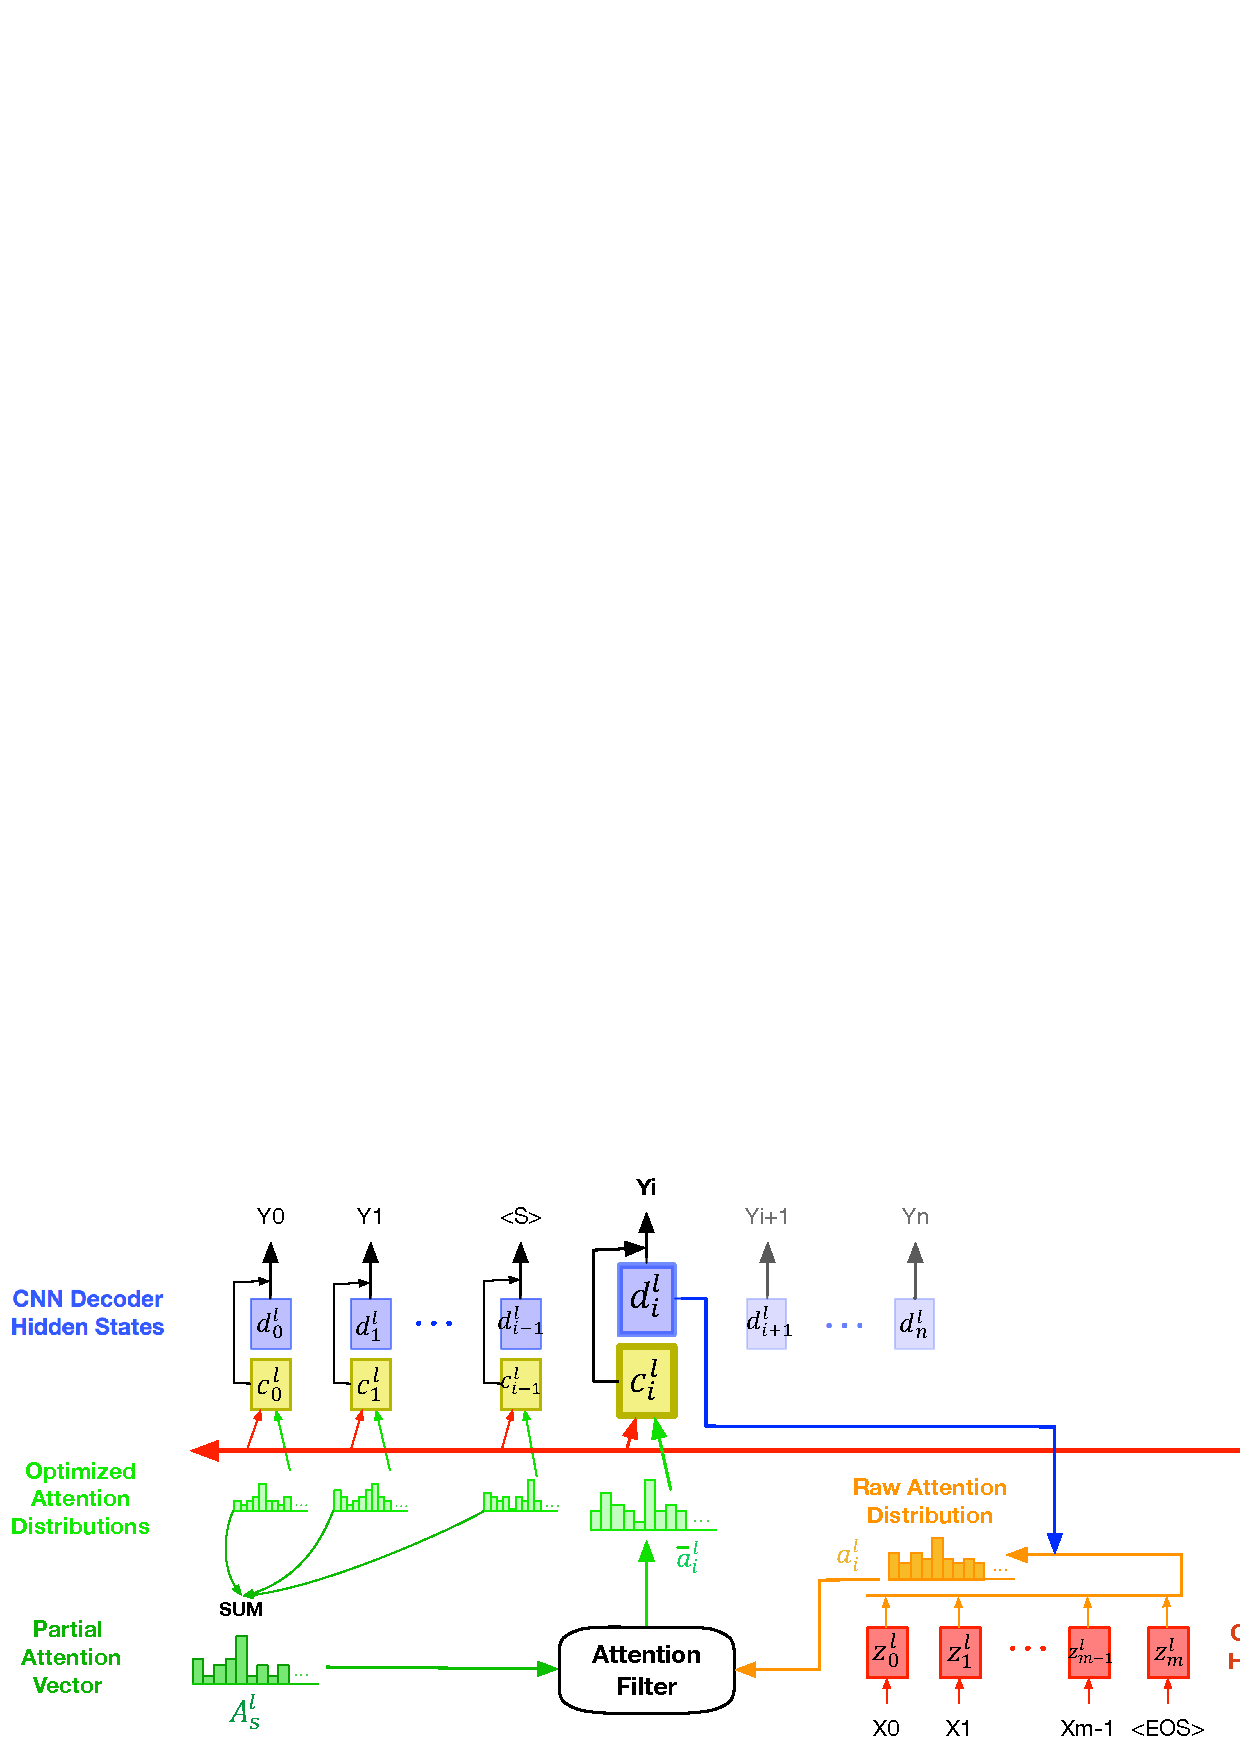
\includegraphics[width=16cm]{model.png}
    \caption{The structure and learning process of the MME framework}
    \label{fig:model}
\end{figure*}
%\KZ{Make figure \ref{fig:model} bigger, fonts bigger too. OK}
In this section, we describe our proposed MME framework in detail.
The MME framework is a novel meta-learning framework which enhances metric-learning based meta methods with a supplementary classifier scheduled by a fast-slow learner strategy. The structure and learning procedure of the MME framework is illustrated in Figure \ref{fig:model}. In \ref{sec:structure} we present the structure of the MME framework. In \ref{sec:process} we show MME's meta-learning process.
\subsection{The structure of MME}
\label{sec:structure}
As is shown in \ref{fig:model}, the structure of MME framework consists of three main parts: context encoder, class matching and supplementary classifier.
\subsubsection{Context encoder}
A support or query instance can be represented as a triple $(s, e, r)$, where $s$ is the sentence containing two entities $e=(e_1,e_2)$, and $r$ is the relation between $e_1$ and $e_2$. $r \in R$ where $R=\{r_1,...,r_N\}$ is the set of all candidate relation classes within one task and $N$ is the number of candidate classes.
Sentence $s=\{c_0,..., c_i, ... c_{T-1}\}$ is of length $T$, where $c_i$ represent the one-hot vector of the $i^{th}$ character.
In context encoder, each $c_i$ is mapped into a $d_c$ dimensional character embedding $\bm{x_i}$.
To integrate positional information of $e_1$ and $e_2$ to each character, for each $c_i$, which is $d_1^i$ and $d_2^i$ characters away from $e_1$ and $e_2$ respectively, we map $d_1^i$ and $d_2^i$ to $d_p$ dimensional position embeddings $\mathbf{d}_1^i,\mathbf{d}_2^i$.
$c_i$ is finally represented as the concatenation of the character embedding and the position embeddings. I.e., $\mathbf{u}_i=[\mathbf{x}_i,\mathbf{d}_1^i,\mathbf{d}_2^i]$.
The representation matrix of sentence $s$ can be written as $\mathbf{U}=[\mathbf{u}_0,..., \mathbf{u}_i, ... ,\mathbf{u}_T]$, which is the concatenation of the representation vectors of the characters. $\mathbf{U} \in \mathbb{R}^{T\times (d_c + 2  d_p)}$.

$\mathbf{U}$ is further fed into an encoder, aiming to extract underlying semantics of sentence $s$. Conventional encoders include convolutional neural networks (CNNs) \citep{LecunBackpropagation} and long short-term memories (LSTMs) \citep{HochreiterLong}. Encoders aggregated with attention have been proposed in recent years. During implementation, we follow \citet{ye-ling-2019-multi}, which facilitates the CNN encoder with local and instance-level attention. The output of the encoder (after pooling) can be symbolled as $\mathbf{E} \in \mathbb{R}^{d_h}$ where $d_h$ is the number of the hidden states.

Thus, an instance can be represented as a pair containing its representation vector $\mathbf{E}$ and relation $r$, i.e., $(\mathbf{E},r)$.


\subsubsection{Class matching}
For each relation $r_i \in R$, the support set $S$ contains a subset of $K$ instances of relation $r_i$, represented as $S^i=\{(\mathbf{E}^1,r_i),...,(\mathbf{E}^K, r_i)\}$. A centroid $\mathbf{C}^i$ is calculated with some aggregation function $\mathcal{A}$ over $S^i$, i.e., $\mathbf{C}^i=\mathcal{A}(\mathbf{E}^1, ..., \mathbf{E}^K)$ and $\mathbf{C}^i \in \mathbb{R}^{d_h}$.

Given an encoded query instance $Q=(\mathbf{E}^q, r^q)$ where $r^q$ is to be predicted, class matching aims to match $r^q$ with some relation class $r_i \in R$. In class matching, conventionally, a function $\mathcal{D}$ is adopted to measure the distance between $\mathbf{E}^q$ and each centroid $\mathbf{C}^{i}$. 
Relation class $r_i$ is chosen as the prediction class if $\mathbf{C}^i$ has the closest distance to $E^q$, i.e., $min(\{\mathcal{D}(\mathbf{E}^q, \mathbf{C}^{j})\}_{j=1}^N)=\mathcal{D}(\mathbf{E}^q, \mathbf{C}^{i})$.
%The relation $r_i$ with the closest distance $\mathcal{D}(\mathbf{E}^q, \mathbf{C}^{i})$ is chosen as the matched relation class.


%The function of class matching is to match an encoded query instance $(\mathbf{E}^q, r^q)$ to a certain class in $R$ given the encoded support set $S$. $S$ can be divided into $N$ subsets according to the relation class of instances: $S=\{S^{1},...,S^{N}\}$ where $S^{i}$ is the set of all instances in the support set with relation $r_i$. $S^{i}=\{(\mathbf{E}^{i}_1, r_i),...,(\mathbf{E}^{i}_K, r_i)\}$ where $r^i \in R$ and $K$ is the number of instances per relation class in the support set. In metric-learning based meta-learning methods, class matching is chiefly conducted by calculating the distance between support vectors and query vectors. Thus, no parameters are contained in this component.

%For the representation vectors $\{\mathbf{E}_1^i, ..., \mathbf{E}^i_K\}$ with the same relation $r_i$, a centroid $\mathbf{C}^i$ is calculated with some aggregation function $\mathcal{A}$, i.e $\mathbf{C}^i=\mathcal{A}(\mathbf{E}_1^i, ..., \mathbf{E}_K^i)$.
%For a query vector $\mathbf{E}^q$, a distance function $\mathcal{D}$ is adopted to calculate the distance between $\mathbf{E}^q$ and each centroid $\mathbf{C}^{i}$. The relation $r_i$ with the closest distance $\mathcal{D}(\mathbf{E}^q, \mathbf{C}^{i})$ is chosen as the prediction.

A naive way of choosing $\mathcal{A}$ and $\mathcal{D}$ is to use mean function and Euclidean distance \citep{proto} respectively. During implementation, we follow \citet{ye-ling-2019-multi} to make $\mathcal{A}$ a weighted sum function and adopt their proposed class-level matching function.

\subsubsection{Supplementary classifier}
To further explore knowledge within support instances, we introduce a supplementary classifier. The supplementary classifier receives representation vector $\mathbf{E}$ of each support instance as input and outputs the the probability of the support instance belonging to each relation class. %to distinguish the relation class $r$ of each support vector $\mathbf{E}$.
The output $\mathbf{O}$ equals to
\begin{eqnarray}
\mathbf{O} &=& \frac{exp(\mathbf{X}_i)}{\sum_{j=0}^{N} exp(\mathbf{X}_j)}, \\
\mathbf{X} &=& \mathbf{WE}+ \mathbf{b},
\end{eqnarray}
where $\mathbf{W}$ and $\mathbf{b}$ are parameters to be trained.

The supplementary classifier aims to reinforce the context encoder by extracting useful information within the support instances. The classifier is active during the training process while is removed while testing. The training procedure with the supplementary classifier is introduced in \ref{sec:process}.

\subsection{The meta learning process}
\label{sec:process}

%\KZ{Too many requires in the algo... Combine them into one require. OK}
\begin{algorithm}[h]
\small
\caption{Meta-Learning Algorithm of MME}\label{alg:metal}
\hspace*{0.02in}{\textbf{Require:}}
distribution over relations in training set $p(\mathcal{R})$,
%\hspace*{0.02in}{\textbf{Require:}}
context encoder $\mathcal{E}_{\theta_0}$,
%\hspace*{0.02in}{\textbf{Require:}}
class matching function $\mathcal{F}$,
%\hspace*{0.02in}{\textbf{Require:}}
supplementary classifier $\mathcal{G}_{\theta_1}$,
%\hspace*{0.02in}{\textbf{Require:}}
fast learner learning rate $\alpha$,
%\hspace*{0.02in}{\textbf{Require:}}
slow learner learning rate $\beta$,
%\hspace*{0.02in}{\textbf{Require:}}
step size $\epsilon$, \#relations per task $N$
\begin{algorithmic}[1]
\State Randomly initialize task-specific parameters $\theta_0$
\State Randomly initialize task-agnostic parameters $\theta_1$
\State Data augmentation if necessary
\label{adddata}
\State $episode\_count=0$
\While {not done}
\State Initialize slow loss $\mathcal{L}_{slow}=0$
\For {$j=1$ to $\epsilon$}
\State $episode\_count++$
\State Sample $N$ relations $\mathcal{R}_i \thicksim p(\mathcal{R})$
\label{sampler}
\State Sample instances $\mathcal{H}=\{s^{(i)}, e^{(i)}, r^{(i)}\}$ from $\mathcal{R}_i$
\label{samplei}
\State Evaluate $\mathcal{L}_{sup}(\mathcal{E}_{\theta_0}, \mathcal{G}_{\theta_1})$ using $\mathcal{H}$
\label{Lsup}
\State Evaluate $\mathcal{L}_{match}(\mathcal{E}_{\theta_0}, \mathcal{F})$ using $\mathcal{H}$
\State Fast loss $\mathcal{L}_{fast}=\mathcal{L}_{sup}$
\label{fastloss}
\State $\mathcal{L}_{slow} = \mathcal{L}_{slow} + \mathcal{L}_{sup} + \mathcal{L}_{match}$
\label{slowloss}
%\State $\mathcal{L}_{slow} = \mathcal{L}_{slow} + \mathcal{L}_{fast}(e_{\theta_0}, g_{\theta_1}) + \mathcal{L}_{fast}(emb_{\theta_0}, f)$
\State $\theta_0 = \theta_0 - \alpha \bigtriangledown_{\theta_0} \mathcal{L}_{fast}$
\label{fast}
\EndFor
\State $\theta_1 = \theta_1 - \beta \bigtriangledown_{\theta_1} \mathcal{L}_{slow}$
\label{slow}
\EndWhile
\State Use $\mathcal{E}_{\theta_0}$ and $\mathcal{F}$ to perform classification of test set.
\label{test}
\end{algorithmic}
\end{algorithm}

The meta-learning process of MME is shown in Algorithm \ref{alg:metal}.
As is in metric-learning based meta-learning, the training process aims to learn a distribution among all the relations. In MME, we propose a novel training algorithm to aggregate a meta-learner into the training process.

Data augmentation is necessary under circumstances where training data is limited(line \ref{adddata}). Common language is required between supplementary data and the training set despite the domain. During training, tasks sampled from original training set is firstly fed into the model. Then, tasks containing classes from both training set and supplementary data are selected. This data aggregation method simulates the the process of learning from the simple to the deep. Experiments show meta-learning can exploit the underlying knowledge in sentences of various domain to achieve gains in performance.

In meta learning, the training process contains multiple episodes. For each episode, a task is randomly generated from the training data (line \ref{sampler} \ref{samplei}).
During the training process of MME, we train two learners: a fast learner with learning rate $\alpha$ and a slow learner with learning rate $\beta$.
The fast learner learns the parameters of the supplementary classifier which are task-specific, and learns after each episode (line \ref{fast}). The objective function of the fast learner (i.e., of the supplementary classifier) is cross entropy loss(line \ref{Lsup} \ref{fastloss}):
\begin{equation}
\begin{aligned}
    \mathcal{L}_{fast} = \mathcal{L}_{sup}= - \sum_{i=1}^{N} \mathbf{r}_i log(\mathbf{O}_i), \\
\end{aligned}
\end{equation}
where $N$ is the number of candidate relation classes, $\mathbf{r}$ is the ground truth one-hot label and $\mathbf{O}$ is the output of the supplementary classifier.
After multiple episodes, the fast learner gains the ability to quickly adapt to new tasks.


For the slow learner which learns parameters of the context encoder, the objective function (line \ref{slowloss}) can be written as:
\begin{equation}
\mathcal{L}_{slow} = \mathcal{L}_{fast} + \mathcal{L}_{match},
\end{equation}
where $\mathcal{L}_{match}$ is the objective function inherited from the core model which provides the context encoder and the class matching function. $\mathcal{L}_{slow}$ accumulates during every $\epsilon$ episodes and then back propagates (line \ref{slowloss} \ref{slow}). Updating parameters regarding to performances of multiple tasks makes the context encoder globally sound.

Thus, after training, we get a supplementary classifier which can quickly adapt to new classification tasks and a global context encoder that fits all tasks. During testing, we only adopt the context encoder to encode the instances and use the distance-based classifier to make predictions (line \ref{test}).

\section{Evaluation}
 We present the basic statistics of our dataset in the first part, and then we evaluate the accuracy of our alignment and annotation process to ensure their reliability. Additionally, we not only test our dataset on different advanced models but also do ablation experiment on both modality and relations annotation. To discover interesting topics about personality dynamics, we focus on those changes of personality and discover several interesting psychological phenomenons.

\subsection{Dataset Statistics}

As we mentioned before, PersonaMovs is not only a large dataset containing a huge amount of text, audio and video corpus but also its data is highly diverse in terms of personality types, movie and television production genres, and relationship types. Fig \ref{Fig:Relats} are the distribution of two types of relations, which indicates the diversity in terms of interaction scenarios.

\begin{figure}[ht]
    \centering
    \includegraphics[width=0.75\linewidth]{images/relations.png}
    \caption{Distribution of social and emotion relations}
    \label{Fig:Relats}
\end{figure}


\subsubsection{Algorithm Evaluation}

To evaluate the performance of our character-to-subtitle matching algorithm, we randomly sample a test case comprising over 50 dialogues and 600 utterances from a variety of genres, including 10 films and TV series. We manually check the aligned characters' name based on the script. Our primary metrics for assessment is accuracy. The algorithm demonstrates an accuracy of about 88\%, indicating a high level of accuracy in correctly identifying character names within subtitles across diverse content types. Compared to existing ASR matching algorithm, our approach gains an improvement by 5\% in accuracy. Besides, our algorithm shows a very strong efficiency comparing the ASR method, of which accelerating almost 7 times.

\begin{table}[ht]
    \small
    \centering
    \begin{tabular}{lllc}
        \hline
        \textbf{Method} & \textbf{Movies} & \textbf{TV} & \textbf{Exec. Time (s)}\\
        \hline
        Gentle (ASR) & 82.71\% & 85.21\% & 26.51\\
        \hline
        Our algorithm & 87.53\% & 88.98\% & 3.55\\
        \hline
    \end{tabular}
    \caption{Accuracy and running time per dialogue of subtitle matching algorithm}
\label{table:alg_eval}
\end{table}

\subsubsection{Annotation Accuracy}
Using ChatGPT to annotate relations for the characters is not a completely worthwhile method. To measure the automatic annotation accuracy, we sampled 235 scenes randomly and involved 5 human labelers on relations annotation. These labelers are in their mid-twenties, 
undergraduate or higher education background, proficient in English with majors in psychology, filmography and sociology, who were instructed to select one of the designated social and emotion relations after aligned video. We continue to compare the automatically annotated results to the human-labeled ground truth. The outcome shows that both social and emotional relationship annotations are dependable, with the accuracy reaching 95\% and 84\% respectively.

\begin{table}[ht]
    \centering
    \small
    \begin{tabular}{llll}
        \hline
        \textbf{Task} & \textbf{Movies} & \textbf{TV} & \textbf{Total}\\
        \hline
        Social Relations& 98.21\% & 93.91\% & 95.78\%\\
        \hline
        Emotion Relations& 82.04\% & 84.46\% & 84.01\%\\
        \hline
    \end{tabular}
    \caption{Accuracy of relations annotation.} 
\label{table:annota_eval}
\end{table}

The dataset's foundation on crowdsourced voting allows for an in-depth analysis of subjective biases in personality perception. Researchers can investigate how different demographics (age, gender, cultural background) perceive personality traits and emotions in characters, revealing biases that may exist in personality assessment. This could also extend to studying the impact of viewer's own personality traits on their perceptions of characters, thus contributing to a deeper understanding of projection and identification processes in media consumption.

\subsection{Experiment Results}
\subsubsection{Dataset Difficulties}
We test our dataset on popular models including BERT~\citep{devlin2019bert}, D-DGCN~\citep{yang2023orders}, Roberta~\citep{liu2019roberta}, AttRCNN~\citep{article1}, GPT-3.5~\citep{openai2023gpt35}, GPT-4~\citep{GPT-4-0125} and MCT~\citep{10386376}. Table \ref{table:Method_Comparison} shows the accuracy of our dataset is apparently lower than other competing datasets. One of the main challenges we observed was the complexity and diversity of our dataset compared to other multimedia datasets. 


\begin{table}[ht]
    \centering
    \small
    \begin{tabular}{lllll}
        \hline
        \textbf{Method} & \textbf{Modalities} & \textbf{FP} & \textbf{TVQA} & \textbf{PM} \\
        \hline
        BERT & T only& 61.14 & 60.61 & \textbf{52.94} \\
        \hline
        D-DGCN & T only & 69.56 & 70.21 & \textbf{68.47} \\
        \hline
        Roberta& T only &62.58 & 69.24 & \textbf{60.37} \\
        \hline
        AttRCNN & T only& 65.01 & 67.25 & \textbf{62.44}\\
        \hline
        GPT-3.5 & T only & 69.21 & 66.89 & \textbf{64.08}\\
        \hline
        GPT-4 & T \& V & 79.14 & 78.33 & \textbf{76.90}\\
        \hline
        MCT & T, A \& V & 71.67 & 69.93 & \textbf{68.47} \\
        \hline
    \end{tabular}
    \caption{Accuracy of different methods on Friends Persona (FP), TVQA, and PersonaMovs (PM). T, A, \& V stand for text, audio and video respectively. Lowest accuracy in each row is bolded.} 
\label{table:Method_Comparison}
\end{table}
A more challenging dataset, such as the one we have developed, offers several advantages in terms of personality detection: 1) Our dataset captures a wide range of real-life situations and intricate contexts, which better mirrors the complexity of human interactions. This realism is crucial for developing models that can perform well in practical applications. 2) Training on a more difficult dataset forces models to learn more nuanced patterns and relationships, leading to better generalization capabilities. 3) A difficult dataset sets a high standard for model evaluation, ensuring that only the most effective models are considered successful. This helps in distinguishing truly advanced models from those that perform well only on simpler tasks. Additionally, one notable observation from the results is that the MCT model, which leverages three modalities (text, audio, and video), does not outperform the GPT-4 model, which uses only two modalities (text and video). This performance gap suggests that Large Language Model outperforms the small model on this task, even though the latter uses more modalities.
\subsubsection{The Importance of Multi-Modality}
\begin{figure*}[ht]
    \centering
    \includegraphics[width=\textwidth, trim= 0 10 0 0, clip]{images/Dynamics.pdf}
    \caption{Case study for personality dynamics.}
    \label{fig:dynamics}
\end{figure*}


We conducted a series of ablation experiments to assess the impact of different modalities and relations annotations on the performance of personality prediction models. The experiments were designed to understand how the exclusion of specific modalities or relations annotations affects the overall prediction accuracy.

\begin{table}[ht]
    \small
    \centering
    \begin{tabular}{c|c|c}
        \hline
        \textbf{Method} & \textbf{Modality} & \textbf{Accuracy}\\
        \hline
        \multirow{4}{*}{MCT} & T \& A & 66.13  \\
        & T \& V & 67.91 \\
        & T only & 63.43 \\
        & T, A \& V & 68.47 \\  
        \hline
        \multirow{2}{*}{GPT-4-0125} & T only & 70.20 \\     
        & T \& V & 76.90 \\
        \hline
    \end{tabular}
    \caption{Ablation experiment on different modalities} 
\label{table:Ablation_modal}
\end{table}


Table \ref{table:Ablation_modal} presents the results of ablation experiments where different combinations of video and audio modalities were excluded. The result underscore the critical importance of using multiple modalities to achieve higher accuracy in personality prediction tasks. Models that leverage both audio and video data, in addition to text, consistently outperform those that rely solely on textual data. 
\begin{table}[ht]
    \centering
    \small
    \begin{tabular}{ccc}
        \hline
        \textbf{Method} & \textbf{With Relations} & \textbf{Without Relations} \\
        \hline
        BERT & 53.88 & 52.94 \\
        \hline
        Roberta & 59.21 & 58.39 \\
        \hline
        GPT-4-0125 & 73.22 & 70.20 \\  
        \hline
    \end{tabular}
    \caption{Ablation experiment on relations annotations.}
    \label{table:Ablation_relationship}
\end{table}

Table \ref{table:Ablation_relationship} shows the results of ablation experiments focusing on the inclusion or exclusion of relations' annotations which finds the relations annotations tend to slightly enhance the performance. This highlights the importance of including rich contextual information to improve the accuracy of personality prediction models. 


The multimodal nature of the dataset (incorporating video, audio, textual, and crowd-sourced data) enables comprehensive studies that integrate different data types to understand personality. This could lead to the development of new theories or the refinement of existing ones that account for the complexity of personality as depicted through various media. It could also foster interdisciplinary research, combining insights from psychology, computer science, linguistics, and media studies.
\subsubsection{Personality Dynamics}

Movies and TV series and their characters often evolve over time, offering a fertile ground for studying personality dynamics. The dataset allows for longitudinal studies on how characters' personalities change in response to narrative events, relationships, and challenges. This could lead to new models that explain personality development and dynamics in complex social settings, bridging narrative theory and psychological research. 

We manually select two famous characters to find their potential change of personality, and we discover there are two types of personality shifts. In the short term, people show different personalities depending on their relations with interlocutor. For example, as shown in Figure \ref{fig:dynamics}, Jay Gatsby from the famous romantic movie called ``\textit{The Great Gatsby}'' behaves as an INFJ in front of his beloved Daisy and as an ENFJ in front of his business partners. In the long term, people may change their personality due to major turning point of life. Like Mia Dolan in ``\textit{La La Land}'', she was always ENFJ, but after the breakup she became an ISFJ. The prediction results generated by GPT-4 align with the peaks in the voting distribution, indicating that this personality shift is observable within our realistic dataset.

According to our finding, we conduct statistical analysis based on our dataset to figure out if there exists certain personalities that are easily attracted to each other. To analyze the patterns of personality attraction, we focus on identifying pairs of personalities that frequently appear together bi-directionally in fondness, aversion, romantic and friendship relations. Figure \ref{fig:networks} presents the favorite network with 16 MBTI personality types, providing a clear visual summary of statistical findings. The size of each node is proportional to the number of connections (degree) it has, which means personality types with more relationships are represented by larger nodes. The color of the edges represents the weight of the relationship between the personality types. Darker edges indicate a higher frequency or stronger relationship. 
%Based on these vivid figures, we can discover very interesting psychological phenomenons. 
For instance, ISTP is the most popular personality since almost every other personality has a fondness relation with it, and ESTP prefers to be around ESFP, ENFP and people with the same personality as themselves. ESFP may not like people with same personality.
% because it has a dark circle on itself.


\begin{figure}[!h]
    \centering
    \begin{subfigure}[b]{0.22\textwidth} 
        \centering
        \includegraphics[width=\linewidth, scale=0.7]{images/fondness.png} 
        \caption{Fondness}
        \label{fig:subgraph1}
    \end{subfigure}
    \hfill
    \begin{subfigure}[b]{0.22\textwidth} 
        \centering
        \includegraphics[width=\linewidth, scale=0.7]{images/dislike.png}
        \caption{Aversion}
        \label{fig:subgraph2}
    \end{subfigure}
    \hfill
    \begin{subfigure}[b]{0.22\textwidth} 
        \centering
        \includegraphics[width=\linewidth, scale=0.7]{images/romantic.png}
        \caption{Romantic}
        \label{fig:subgraph3}
    \end{subfigure}
    \hfill
    \begin{subfigure}[b]{0.22\textwidth} 
        \centering
        \includegraphics[width=\linewidth, scale=0.7]{images/friendship.png} 
        \caption{Friendship}
        \label{fig:subgraph4}
    \end{subfigure}
    \caption{Favorite Networks with Different Personalities about Four Relations}
    \label{fig:networks}
\end{figure}

By including data on social and emotion relations between characters, the dataset opens new pathways for exploring the dynamics of personality through interactions. This aspect can support research into how different personality types influence and are influenced by social networks, both within narrative contexts and long-term conversions. It provides a basis for computational models that simulate personality dynamics in social networks, potentially informing theories on social behavior, conflict resolution, and group dynamics.

\section{Conclusion}

In this study, we conducted a comprehensive analysis of Prison Term Prediction (PTP) and identified two major issues: structural representation of legal knowledge and the scarcity of training data for most crimes. To address these issues, we proposed a novel approach, \lawgraph{}, to represent the structural legal knowledge. We further proposed a lightweight Statute Knowledge Encoder (SKE) for end-to-end training of our model. We performed extensive experiments to compare SKE with previous works and LLMs. The experimental results have indicated the superiority of SKE over previous works. 

\section*{Ethical Statements}

Copyright © [2024] by the authors. The movies and TV series included in this dataset are copyrighted by their respective copyright owners and are used in this work for academic and research purposes under fair use guidelines or specific permissions obtained from the copyright holders. This does not imply endorsement by or affiliation with the copyright owners. Use of these materials is limited to the scope of the permission granted and is not intended for commercial distribution.


\section*{Limitations}
While our PersonaMosaic designed for personality prediction shows superiority in most aspects, it also comes with inherent limitations.

Dialogues and character behaviors extracted from movies or TV shows may not always accurately reflect real-life personality traits due to the scripted nature of these interactions. Fictional characters are often designed to serve a narrative purpose, which might exaggerate or oversimplify certain personality traits for dramatic effect, leading to potential biases in personality prediction.

The process of annotating dialogues, character relationships, and personality traits, even if partially automated, involves a degree of subjectivity. Different annotators might interpret the same dialogue or behavior differently based on their own biases and experiences, leading to inconsistencies in the dataset.

The dataset may predominantly reflect the cultural norms and values of the society in which the content was produced, potentially limiting its applicability across different cultural contexts. Our dataset is based on English movies and TV shows, so it may not interpret other non-English cultural contexts properly.


\bibliography{custom}

\appendix
\section{Definitions of Personality Models}
\label{sec:appendixA}

\begin{itemize}
  \item \textbf{Myers–Briggs Type Indicator (MBTI)}: The MBTI categorizes personality into four dimensions. Extraversion (E) vs. Introversion (I): Extraverts are outgoing and energized by social interactions, while Introverts are reserved and energized by solitude. Sensing (S) vs. Intuition (N): Sensors focus on present, concrete information, valuing practicality, whereas Intuitives are imaginative and future-oriented, valuing abstract ideas. Thinking (T) vs. Feeling (F): Thinkers base decisions on logic and fairness, prioritizing objectivity, while Feelers base decisions on personal values and the impact on others, prioritizing harmony. Judging (J) vs. Perceiving (P): Judgers prefer structured and organized lives, liking plans and decisiveness, while Perceivers prefer flexibility and spontaneity, liking to keep their options open. Each MBTI type is defined by a combination of four cognitive functions, which can be either introverted (i) or extraverted (e). Extraverted Sensing (Se): Focuses on the present moment and physical reality, highly attuned to sensory experiences. Introverted Sensing (Si): Relies on past experiences and memories, valuing tradition and consistency. Extraverted Intuition (Ne): Sees patterns and connections, focusing on future possibilities and abstract ideas. Introverted Intuition (Ni): Focuses on internal insights and foresight, seeing underlying meanings and future potentials. Extraverted Thinking (Te): Organizes and structures the external world, prioritizing logic and efficiency. Introverted Thinking (Ti): Analyzes and categorizes information internally, valuing logical consistency and understanding. Extraverted Feeling (Fe): Prioritizes harmony and social values, focusing on the needs and feelings of others. Introverted Feeling (Fi): Values personal beliefs and feelings, making decisions based on inner values and ethics.
  \begin{table*}[ht]
    \centering
    \small
    \begin{tabular}{ll}
      \hline
      \textbf{Relations type} & \textbf{Description}\\
      \hline
      Family & Parents (grandparents) and children, siblings, etc.\\
      \hline
      Friendship & Based on common interest, mutual respect and affection, but not related to the blood.\\
      \hline
      Romantic & Based on emotional attraction and include dating, marriage, etc.\\
      \hline
      Professional & Formed in a work environment, such as colleagues, superiors and subordinates, etc.\\ 
      \hline
      Social & Formed in a broader social context, such as neighbors, club members.\\
      \hline
      Academic & Formed in an educational setting, such as between teachers and students, classmates.\\
      \hline
      Online & Established in online spaces or through social media platforms.\\
      \hline
    \end{tabular}
    \caption{Descriptions of Social Relations}
    \label{table:social}
    \end{table*}
    
    \begin{table*}[ht]
      \small
      \centering
      \begin{tabular}{ll}
        \hline
        \textbf{Relations type} & \textbf{Description}\\
        \hline
        Fondness & A positive emotion characterized by a person's fondness for another.\\
        \hline
        Jealousy & Unhappy and angry because someone has something that you want.\\
        \hline
        Aversion  & A negative emotion, referring to a feeling of disfavor towards someone.\\
        \hline
        Pity  & A feeling of sadness for someone else's difficult situation.\\ 
        \hline
        Respect & Admiration felt or shown for someone that you believe has good ideas or qualities.\\
        \hline
        Hostility  & An unfriendly or unkindness towards someone or something.\\
        \hline
        Envy & A discontented feeling when a person desires what someone else has.\\
        \hline
        Gratitude & An emotion of being thankful for someone else's help or kind actions.\\
        \hline
      \end{tabular}
      \caption{Description of Emotion Relations}
      \label{table:emotional}  
    \end{table*}
  \item \textbf{Big Five Personality Traits}: The Big Five model describes personality using five broad traits. Openness to Experience: High openness involves imagination and insight, while low openness involves practicality and routine. Conscientiousness: High conscientiousness is characterized by organization and dependability, while low conscientiousness is characterized by spontaneity and flexibility. Extraversion: High extraversion includes sociability and assertiveness, while low extraversion (introversion) includes reserve and solitude. Agreeableness: High agreeableness involves trust and altruism, while low agreeableness involves skepticism and competition. Neuroticism: High neuroticism involves emotional instability and anxiety, while low neuroticism involves emotional stability and calmness.
  \item \textbf{Enneagram}: The Enneagram classifies personality into nine types, each representing different motivations and fears. Type 1: The Reformer, driven by a need for perfection. Type 2: The Helper, driven by a need to be loved. Type 3: The Achiever, driven by a need for success. Type 4: The Individualist, driven by a need for uniqueness. Type 5: The Investigator, driven by a need for knowledge. Type 6: The Loyalist, driven by a need for security. Type 7: The Enthusiast, driven by a need for variety and fun. Type 8: The Challenger, driven by a need for control. Type 9: The Peacemaker, driven by a need for harmony. A 2w3 individual is likely to be more ambitious, charming, and goal-oriented than a typical Type 2. They still seek to help others but are also motivated by a desire for success and recognition.
  \item \textbf{Instinctual Variants}: The Instinctual Variants theory describes three primary instinctual drives influencing behavior. Self-Preservation (SP): Focuses on safety, health, and comfort. Social (SO): Focuses on relationships, status, and community. Sexual (SX): Focuses on intimacy, attraction, and one-on-one connections. For instance, an 8w7 with a Sexual variant, is highly charismatic and seeks intense and passionate connections with others. He or she is bold and assertive, often focusing his or her energy on building strong, impactful relationships.
\end{itemize}

\section{Definitions of Relations}
\label{sec:appendixB}
Human social networks are complex and multifaceted. By categorizing relations, we can better understand the dynamics and nuances of how people interact with each other. Different types of relations provide context for interactions, which is crucial for analyzing social behaviors and patterns, improving social network analysis, and applying this knowledge across various fields and applications.
Table \ref{table:social} and Table \ref{table:emotional} provide a structured approach to understanding the complex web of relations that individuals navigate. By categorizing these relations into social and emotional types, we can better analyze and predict personality dynamics in various contexts~\citep{Collins_Sroufe_1999, 10.1093/acprof:oso/9780195150100.001.0001}. 



\section{Data Alignment Algorithm}
\label{sec:appendixC}
The details of data alignment algorithm are as follows:
\begin{algorithm}[!h]
	\small
	\caption{Scripts and Subtitles Matching}
	\label{alg:Matching}
	\renewcommand{\algorithmicrequire}{\textbf{Input:}}
	\renewcommand{\algorithmicensure}{\textbf{Output:}}
	
	\begin{algorithmic}[1]
		\REQUIRE $Script, Subtitles$
		\ENSURE Updated subtitles with speaker names
		\STATE $dial \& speakers \gets empty$
		\STATE $threshold \gets 0.8$
		\FOR{$scene$ in $Script$}
		\FOR{$Dials$ in $scene$}
		\STATE Extract $speaker$ and $dial$ from $Dials$
		\STATE $dial \& speakers \gets speaker, dial$ 
		\ENDFOR
		\ENDFOR
		\FOR{$subtitle$ in $Subtitles$}
		\STATE $match\_score \gets 0$
		\STATE $match\_speaker \gets Null$
		\FOR{$line$ in $subtitle$}
		\FOR{$speaker, dial$ in $dial \& speakers$}
		\STATE $score \gets Similar(subtitle, dial)$
		\IF{$score$ > $match\_score$}
		\STATE Update $match\_score$ and $match\_speaker$
		\ENDIF
		\ENDFOR
		\IF{$match\_score \geq threshold$}
		\STATE Update $line$ with $match\_speaker$
		\ENDIF
		\ENDFOR
		\STATE Update $subtitle$
		\ENDFOR
		\RETURN Updated $Subtitles$
	\end{algorithmic}
\end{algorithm}

\begin{enumerate}
      \item \textit{Preprocess the raw data} Firstly, we divide the scripts into several scenes according to the coherence in language of camera, instead of randomly clipping in a certain time period. This segmentation is guided by explicit scene transition cues found in movie scripts, such as ``\textit{CUT TO:}'' or scene location indicators. For TV show scripts, which might lack uniform scene transition markers, we identify scene changes by detecting pauses exceeding 3 seconds between utterances.
      \item \textit{Match the utterance} This algorithm is rooted in the comparison of utterances from original scripts and subtitles based on a similarity threshold. If the similarity between a pair of utterances meets or exceeds this threshold, the character's name is accurately associated with the utterance.
      \item \textit{Rematch with the slide window} Basically, the content in scripts is slightly different with the subtitles, because the director may have improvised on the set. Thus, we introduce a slide window algorithm to evaluate the utterance-level similarity. As shown in Algorithm \ref{alg:window}, we set a window to slide over the script and, for each utterance, compare the content inside the window with each subtitle entry to get the similarity of the paragraph in the window. 
\end{enumerate}

\begin{algorithm}[h]
	\caption{Slide Window Matching}
	\small
	\label{alg:window}
	\renewcommand{\algorithmicrequire}{\textbf{Input:}}
	\renewcommand{\algorithmicensure}{\textbf{Output:}}
	
	\begin{algorithmic}[1]
		\REQUIRE $Script, Subtitles$
		\ENSURE Updated subtitles 
		\STATE $window\_size \gets 10$
		\STATE $threshold \gets 0.8$
		\STATE $matches \gets empty\_list$
		\FOR{$i \gets 0$ to $Len(Script) - window\_size$}
		\STATE $window \gets slice(scriptTokens, i, i + window\_size)$
		\STATE $match\_score \gets 0$
		\FOR{$j \gets 0$ to $Len(Subtitles) - 1$}
		\STATE $score \gets Similar(window, Subtitles[j])$
		\IF{$score$ > $match\_score$}
		\STATE Update $match\_score$
		\ENDIF
		\ENDFOR
		\IF{ $match\_score \geq threshold$}
		\STATE $matches \gets Subtitles[j]$
		\ENDIF
		\ENDFOR
		\RETURN Updated $Subtitles$ with $matches$
	\end{algorithmic}
\end{algorithm}

%\section{Prompt Design}
%\label{appedix:prompt}

\end{document}
